\documentclass[a4paper]{article}
\usepackage{ucs}
\usepackage[utf8x]{inputenc}
\usepackage[T1]{fontenc}
\usepackage{german}
\usepackage{a4,ngerman}
\usepackage[ngerman]{babel}
\usepackage{graphicx}
\usepackage[]{cite}
\usepackage{fancyhdr}
\pagestyle{fancy}
\selectlanguage{german}
\usepackage{array}
\usepackage{lastpage}
\usepackage{listings}
\usepackage{color}

\lhead{ALG1 und PRG1}
\chead{Lukas Schörghuber}
\rhead{Übung 4}
\cfoot{}
\rfoot{Seite \arabic{page} von \pageref{LastPage}}

\lstset
{
	language=Pascal,
	basicstyle=\small\ttfamily,
	numbers=left,
	numberstyle=\tiny,
	frame=tb,
	showstringspaces=false,
	keywordstyle=\color{blue},
	commentstyle=\color{green},
	stringstyle=\color{red},
	tabsize=2
}

\begin{document}
	\begin{enumerate}
		\item
		\begin{enumerate}
			\item
			\section*{Lösungsidee}
			
			In der Funktion wird zuerst überprüft, ob die Basis kleiner gleich 36 ist. Danach wird der String in einer While-Schleife von hinten nach vorne Zeichen für Zeichen durchlaufen.
			\newline
			Im Rumpf der Vorschleife wird der Wert des Zeichens im Dezimalsystem ermittelt. Anschließend wird überprüft, ob die Basis den Wert des Zeichens zulässt. Falls der Wert größer 0 ist, wird der Wert mit dem Stellenwert multipliziert und zum Ergebnis der Funktion addiert. Der Stellenwert kann durch die Formel $ Basis^{Länge des Eingabestrings - 1} $ ermittelt werden.
			
			\section*{Implementierung}
			\begin{lstlisting}[label=scValueOf_a, resetmargins=true]
CONST MAX_BASE = 36;
  MIN_BASE = 2;
  ASCII_0 = Ord('0');
  ASCII_9 = Ord('9');
  ASCII_A_UPPER = Ord('A');
  ASCII_Z_UPPER = Ord('Z');
  ASCII_A_LOWER = Ord('a');
  ASCII_Z_LOWER = Ord('z');
  ALPHANUMERIC_DIGIT_OFFSET = 10;
  MAX_STRING_REPRESENTATION_LENGTH = 5;

(* Determine base power exponent. *)
FUNCTION Power(base: SMALLINT; exponent: SMALLINT): SMALLINT;
  VAR i: INTEGER;
    result: SMALLINT;
BEGIN
  IF exponent > 0 THEN BEGIN
    result := base;
    FOR i := 2 TO exponent DO BEGIN
      result := result * base;
    END;
    Power := result;
  END
  ELSE BEGIN
    Power := 1;
  END;
END;

(* Convert a lower case ASCII character to upper case. *)
FUNCTION ToUpperCase(characterToConvert: CHAR): CHAR;
  VAR characterASCIIValue: BYTE;
BEGIN
  characterASCIIValue := Ord(characterToConvert);
  (* check if the character is a lower case character *)
  IF
    (characterASCIIValue >= ASCII_A_LOWER)
  AND
    (characterASCIIValue <= ASCII_A_UPPER) THEN BEGIN
    ToUpperCase := Chr(characterASCIIValue - (ASCII_A_LOWER - ASCII_A_UPPER));
  END
  ELSE BEGIN
    ToUpperCase := Chr(characterASCIIValue);
  END;
END;

(* Convert a number in an arbitary base into a decimal number. *)
FUNCTION ValueOf(digits: STRING; base: INTEGER): INTEGER;
  VAR i: INTEGER;
    numberOfDigits: INTEGER;
    processedDigit: BYTE;
    actualDigitASCIIValue: BYTE;
    decimalValue: INTEGER;
    invalidDigit: BOOLEAN;
BEGIN
  (* check if the base is within the allowed range *)
  IF (base >= MIN_BASE) AND (base <= MAX_BASE) THEN BEGIN
    decimalValue := 0;
    numberOfDigits := Length(digits);
    i := Length(digits);
    invalidDigit := FALSE;
    (* process the input string character by character in reverse order (as we can) *)
    WHILE (i >= 1) AND (invalidDigit = FALSE) DO BEGIN
      actualDigitASCIIValue := Ord(ToUpperCase(digits[i]));

      (* check if the character is a number or a letter *)
      IF
        (actualDigitASCIIValue >= ASCII_0)
      AND
        (actualDigitASCIIValue <= ASCII_9) THEN BEGIN
        processedDigit := actualDigitASCIIValue - ASCII_0;
      END
      ELSE IF
        (actualDigitASCIIValue >= ASCII_A_UPPER)
      AND
        (actualDigitASCIIValue <= ASCII_Z_UPPER) THEN BEGIN
        processedDigit := actualDigitASCIIValue - ASCII_A_UPPER
          + ALPHANUMERIC_DIGIT_OFFSET;
      END
      ELSE BEGIN
        (* invalid character detected --> exit the loop *)
        WriteLn('Invalid character "', digits[i],
          '"! Please limit your input to digits and letters.');
        invalidDigit := TRUE;
      END;

      IF invalidDigit = FALSE THEN BEGIN
        (* check if the decimal value is within the allowed range *)
        IF processedDigit < base THEN BEGIN
          IF processedDigit <> 0 THEN BEGIN
            (* add the character multiplied by the base power the significance *)
            decimalValue := decimalValue
              + (processedDigit * Power(base, numberOfDigits - i));
          END;
        END ELSE BEGIN
          (* invalid character detected --> exit the loop *)
          WriteLn('The character "', digits[i], '" exceeds the specified base.');
          invalidDigit := TRUE;
        END;
      END;

      i := i - 1;
    END;

    IF invalidDigit = FALSE THEN BEGIN
      ValueOf := decimalValue;
    END
    ELSE BEGIN
      ValueOf := (-1);
    END;
  END
  ELSE BEGIN
    ValueOf := (-1);
  END;
END;
			\end{lstlisting}
			
			\section*{Testfälle}
			
			Zuerst wird getestet, ob die Funktion bei einer Basis größer als 36 den Wert für Fehler gemäß Spezifikation (-1) zurückliefert. Analog dazu wird ein Test für eine Basis kleiner 2 durchgeführt.
			\begin{center}
				\begin{figure}[ht!]
					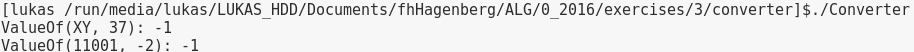
\includegraphics[scale=0.4]{converter/tests/invalidBase.png}
					\caption{Verhalten bei nicht erlaubter Basis}
					\label{tValueOfInvalidBase}
				\end{figure}
			\end{center}
			
			Die Funktion soll ebenfalls in der Lage sein Zeichen deren Wert größer als die Basis ist zu erkennen und -1 zurückzuliefern. Dies ist in Abbildung \ref{tValueOfInvalidCharacters} zu sehen.
			\begin{center}
				\begin{figure}[ht!]
					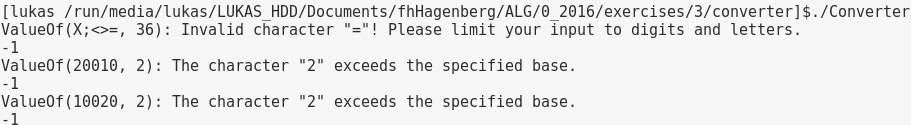
\includegraphics[scale=0.4]{converter/tests/invalidCharacters.png}
					\caption{Verhalten bei nicht erlaubten Zeichen}
					\label{tValueOfInvalidCharacters}
				\end{figure}
			\end{center}
			
			Abschließend wird noch demonstriert, dass die Funktion die Zahlen korrekt umrechnet. Dazu wird eine Eingabe mit der Basis 2, eine Eingabe mit der Basis 36 und eine Eingabe mit der Basis 10 durchgeführt. Wie im unten befindlichen Screenshot ersichtlich ist, liefert die Funktion die richtigen Werte.
			\begin{center}
				\begin{figure}[ht!]
					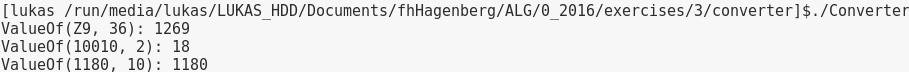
\includegraphics[scale=0.4]{converter/tests/valueOf.png}
					\caption{Korrekte Umrechnungen}
					\label{tValueOf}
				\end{figure}
			\end{center}
			
			\clearpage
			\item
			\section*{Lösungsidee}
			Diese Funktion überprüft zu Beginn ebenfalls, ob die Basis nicht größer als der Maximalwert (36) oder kleiner als der Minimalwert (2) ist.
			
			\section*{Implementierung}
			\begin{lstlisting}[label=scDigitsOf, resetmargins=true]
(* Get the character representation of either a digit or a letter. *)
Function NumberToChar(number: INTEGER): CHAR;
BEGIN
  IF number >= ALPHANUMERIC_DIGIT_OFFSET THEN BEGIN
    NumberToChar := Chr(number - ALPHANUMERIC_DIGIT_OFFSET + ASCII_A_UPPER);
  END
  ELSE BEGIN
    NumberToChar := Chr(number + ASCII_0);
  END;
END;

FUNCTION DigitsOf(value: INTEGER; base: INTEGER): STRING;
  VAR i, j: SMALLINT;
  VAR remainder: INTEGER;
  VAR stringRepresentationReverse: STRING[MAX_STRING_REPRESENTATION_LENGTH];
  VAR stringRepresentation: STRING[MAX_STRING_REPRESENTATION_LENGTH];
BEGIN
  (* check if the base is within the allowed range *)
  IF (base >= MIN_BASE) AND (base <= MAX_BASE) THEN BEGIN
    i := 1;
    (* use the Horner method for storing the digits in reverse order *)
    WHILE (value > 0) DO BEGIN
      remainder := value MOD base;
      stringRepresentationReverse[i] := NumberToChar(remainder);
      value := value DIV base;
      IF value > 0 THEN BEGIN
        i := i + 1;
      END;
    END;

    (* reverse the order of the characters *)
    FOR j := i DOWNTO 1 DO BEGIN
      stringRepresentation[i - j + 1] := stringRepresentationReverse[j];
    END;
    (* set the length of the result string *)
    stringRepresentation[0] := Chr(i);
    DigitsOf := stringRepresentation;
  END
  ELSE BEGIN
    DigitsOf := '';
  END;
END;
			\end{lstlisting}
			
			\clearpage
			\section*{Testfälle}
			Die Überprüfung der Basis wurde bereits in der letzten Funktion dokumentiert. Daher werden im  Screenshot \ref{tDigitsOf} nur die beim Test der Funktion ValueOf ermittelten Ergebnissen wieder in ihre ursprüngliche Form zurückkonvertiert.
			\begin{center}
				\begin{figure}[ht!]
					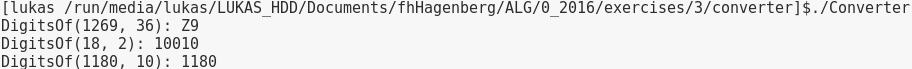
\includegraphics[scale=0.4]{converter/tests/digitsOf.png}
					\caption{Korrekte Umrechnungen}
					\label{tDigitsOf}
				\end{figure}
			\end{center}
			
			\item
			\section*{Lösungsidee}
			Die vier Funktionen zur Abbildung der Grundrechnungsarten verwenden die Funktion ValueOf, um die Zahlen in das Dezimalsystem zu konvertieren und verwenden anschließend die Standardoperatoren, um das Ergebnis zu ermitteln. Das Ergebnis wird jedoch nur ermittelt, wenn die beiden ValueOf-Aufrufe nicht -1 als Ergebnis lieferten. Bei der Division wird zusätzlich überprüft, ob der Divisor nicht 0 ist.
			
			\section*{Implementierung}
			\begin{lstlisting}[label=scCalculation, resetmargins=true]
FUNCTION Sum(d0: STRING; b0: INTEGER; d1: STRING; b1: INTEGER): INTEGER;
  VAR numberA, numberB: INTEGER;
BEGIN
  numberA := ValueOf(d0, b0);
  numberB := ValueOf(d1, b1);
  IF (numberA <> (-1)) AND (numberB <> (-1)) THEN BEGIN
    Sum := numberA + numberB;
  END
  ELSE BEGIN
    Sum := (-1);
  END;
END;

FUNCTION Diff(d0: STRING; b0: INTEGER; d1: STRING; b1: INTEGER): INTEGER;
  VAR numberA, numberB: INTEGER;
BEGIN
  numberA := ValueOf(d0, b0);
  numberB := ValueOf(d1, b1);
  IF (numberA <> (-1)) AND (numberB <> (-1)) THEN BEGIN
    Diff := numberA - numberB;
  END
  ELSE BEGIN
    Diff := (-1);
  END;
END;

FUNCTION Prod(d0: STRING; b0: INTEGER; d1: STRING; b1: INTEGER): INTEGER;
  VAR numberA, numberB: INTEGER;
BEGIN
  numberA := ValueOf(d0, b0);
  numberB := ValueOf(d1, b1);
  IF (numberA <> (-1)) AND (numberB <> (-1)) THEN BEGIN
    Prod := numberA * numberB;
  END
  ELSE BEGIN
    Prod := (-1);
  END;
END;

FUNCTION Quot(d0: STRING; b0: INTEGER; d1: STRING; b1: INTEGER): INTEGER;
  VAR numberA, numberB: INTEGER;
BEGIN
  numberA := ValueOf(d0, b0);
  numberB := ValueOf(d1, b1);
  IF (numberA <> (-1)) AND (numberB > 0) THEN BEGIN
    Quot := numberA DIV numberB;
  END
  ELSE BEGIN
    Quot := (-1);
  END;
END;
			\end{lstlisting}
			
			\section*{Testfälle}
			Zuerst wird überprüft, ob jede der vier Funktionen bei ungültigen Eingaben -1 zurückliefert. Darüber hinaus wird geprüft, ob eine Divison durch 0 als Fehler erkannt wird. Die Ergebnisse (alle -1, d.h. ungültig) sind in Abbildung \ref{calcInvalidInputs} ersichtlich.
			\begin{center}
				\begin{figure}[ht!]
					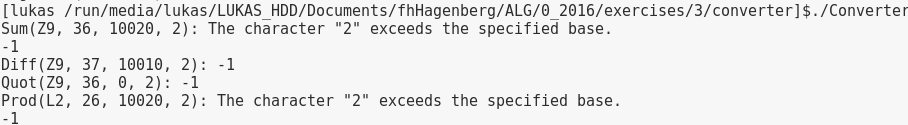
\includegraphics[scale=0.40]{converter/tests/calcInvalidInputs.png}
					\caption{Korrektes Fehlerverhalten bei ungültigen Eingaben}
					\label{calcInvalidInputs}
				\end{figure}
			\end{center}
			
			Zum Abschluss dieser Nummer werden den Funktionen korrekte Eingabewerte übergeben und das Ergebnis stimmt nun ebenfalls.
			\begin{center}
				\begin{figure}[ht!]
					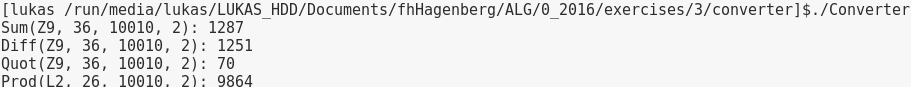
\includegraphics[scale=0.40]{converter/tests/calc.png}
					\caption{Korrekte Ergebnisse der 4 Grundrechnungsarten}
					\label{calc}
				\end{figure}
			\end{center}
		\end{enumerate}
		
		\clearpage
		\item
		Nach der Datentypdefinition eines Records zur Abspeicherung der Ergebnisse einer Umfrage, wird ein Arraytyp definiert, der ein Feld in der Größe einer Konstante abspeichert.
		\newline
		Anschließend wird der Benutzer gebeten, jeweils die negativen als auch die positiven Umfrageergebnisse für die Politiker einzugeben. Nach der Eingabe wird der Absolutbetrag berechnet, was auch negative Eingaben für die Unbeliebtheit eines Politikers ermöglicht. Als Nächstes wird der Wert auf die Zehnerstelle gerundet. Abschließend wird noch überprüft, ob die beiden Werte zusammen kleiner als 100\% sind. In diesem Fall oder bei der Eingabe eines ungültigen Umfragewertes wird das Programm beendet.
		\newline
		Nach der Eingabe werden die Ergebnisse erneut durchlaufen und ausgegeben. Die Ausgabe wird so gestaltet, dass ein Minimum an Platz (im Minimalfall nur der Platz für die Spaltenüberschriften) benötigt wird.
		
		\section*{Implementierung}
		\begin{lstlisting}[resetmargins=true]
PROGRAM Diagram;

CONST POLTICIAN_COUNT = 2;
  PADDING_CENTER = 1;
  HEADER_MIN_LENGTH = 8;
  EXIT_FAILURE = 1;

TYPE PollResult = RECORD
  PositiveVotes: SHORTINT;
  NegativeVotes: SHORTINT;
END;

TYPE PoliticianPollResults = ARRAY[1..POLTICIAN_COUNT] OF PollResult;

VAR politicianPoll: PoliticianPollResults;
  extremeValues: PollResult;

(* Calculates the absolute value of the parameter. *)
FUNCTION Abs(n: INTEGER): INTEGER;
  VAR square: LONGINT;
BEGIN
  square := (n * n);
  Abs := Round(Sqrt(Square));
END;

(* Determines the maximum of the two input parameters. *)
FUNCTION Max2(number_a, number_b: INTEGER): INTEGER;
BEGIN
  IF number_a > number_b THEN BEGIN
    Max2 := number_a;
  END
  ELSE BEGIN
    Max2 := number_b;
  END;
END;

(*
  Rounds a number and returns the result without the trailing 0
  --> divides result by 10.
*)
FUNCTION Round10(number_to_round: INTEGER): INTEGER;
  CONST ROUNDING_ACCURACY = 10;

  VAR digit_post_10, digit_pre_10: INTEGER;
BEGIN
  digit_post_10 := number_to_round MOD ROUNDING_ACCURACY;
  digit_pre_10 := number_to_round DIV 10;
  IF digit_post_10 < 5 THEN BEGIN
    Round10 := digit_pre_10;
  END
  ELSE BEGIN
    Round10 := (digit_pre_10 + 1);
  END;
END;

(*
Reads the result of the poll.

In addition, the input is validated.
Furthermore, the maximum and the minimum values required for displaying purposes are stored.
*)
PROCEDURE DeterminePoliticianRating(VAR pollResult: PoliticianPollResults;
  VAR extremeValues: PollResult);
  CONST NEGATIVE_VOTES_MIN = -100;
    NEGATIVE_VOTES_MAX = 100;
    POSITIVE_VOTES_MAX = 100;
    POSITIVE_VOTES_MIN = 0;

  VAR i: SMALLINT;
BEGIN
  FOR i := 1 TO POLTICIAN_COUNT DO BEGIN
    Write('Please enter the number of negative poll results for politician ', i, '>');
    ReadLn(pollResult[i].NegativeVotes);
    IF
      (pollResult[i].NegativeVotes > NEGATIVE_VOTES_MAX)
    OR
      (pollResult[i].NegativeVotes < NEGATIVE_VOTES_MIN)
    THEN BEGIN
      (* invalid input --> terminate program *)
      WriteLn('Please enter a valid integer between ', NEGATIVE_VOTES_MIN,
        ' and ', NEGATIVE_VOTES_MAX);
      System.Halt(EXIT_FAILURE);
    END;
    pollResult[i].NegativeVotes := Abs(pollResult[i].NegativeVotes);

    Write('Please enter the number of positive poll results for politician ', i, '>');
    ReadLn(pollResult[i].PositiveVotes);
    IF
		  (pollResult[i].PositiveVotes > POSITIVE_VOTES_MAX)
		  OR
      (pollResult[i].PositiveVotes < POSITIVE_VOTES_MIN)
    THEN BEGIN
      (* invalid input --> terminate program *)
      WriteLn('Please enter a valid integer between ', POSITIVE_VOTES_MIN,
        ' and ', POSITIVE_VOTES_MAX);
      System.Halt(EXIT_FAILURE);
    END;
    pollResult[i].PositiveVotes := Abs(pollResult[i].PositiveVotes);

	  (* round the value and retrieve the relevant part (without trailing 0) *)
    pollResult[i].NegativeVotes := Round10(pollResult[i].NegativeVotes);
    pollResult[i].PositiveVotes := Round10(pollResult[i].PositiveVotes);

    IF (pollResult[i].NegativeVotes + pollResult[i].PositiveVotes) > 10 THEN BEGIN
      (* input exceeds 100 per cent --> terminate the program *)
      WriteLn('The two rounded values you entered exceed 100 per cent
        which means the values are invalid.');
      System.Halt(EXIT_FAILURE);
    END;

    (* Determine the extreme values of the total input. *)
    extremeValues.NegativeVotes := 
      Max2(extremeValues.NegativeVotes, pollResult[i].NegativeVotes);
    extremeValues.PositiveVotes :=
      Max2(extremeValues.PositiveVotes, pollResult[i].PositiveVotes);
  END;
END;

(* Prints the correct number of X representing the positive and negative votes. *)
PROCEDURE PrintRow
(
  negative_votes, positive_votes: SMALLINT;
  columnLengthNegative, columnLengthPositive: SMALLINT
);
  VAR i: SMALLINT;
BEGIN
  (* print the negative votes *)
  FOR i := columnLengthNegative DOWNTO 1 DO BEGIN
    IF i = 1 THEN BEGIN
      Write(' ');
    END
    ELSE BEGIN
      IF (i - 1) <= negative_votes THEN BEGIN
        Write('X');
      END
      ELSE BEGIN
        Write(' ');
      END;
    END;
  END;

  Write('|');

  (* print the positive votes *)
  FOR i := 1 TO columnLengthPositive DO BEGIN
    IF i > PADDING_CENTER THEN BEGIN
      IF (i - 1) > positive_votes THEN BEGIN
        Write(' ');
      END
      ELSE BEGIN
        Write('X');
      END;
    END
    ELSE BEGIN
      Write(' ');
    END;
  END;

  WriteLn('');
END;

(* Print the heading naming the left (negative) and right(positive) column. *)
PROCEDURE PrintHeader(columnLengthNegative, columnLengthPositive: SMALLINT);
  VAR i: SMALLINT;
BEGIN
  Write('  ');

  i := columnLengthNegative;
  WHILE i > 0 DO BEGIN
    IF i = 1 THEN BEGIN
      Write(' ');
    END
    ELSE BEGIN
      IF (i - 1) <= HEADER_MIN_LENGTH THEN BEGIN
        Write('negative');
        i := i - (HEADER_MIN_LENGTH - 1);
      END
      ELSE BEGIN
        Write(' ');
      END;
    END;
    i := i - 1;
  END;

  Write(' ');

  i := 1;
  WHILE i <= columnLengthPositive DO BEGIN
    IF i > PADDING_CENTER THEN BEGIN
      IF (i - 1) > HEADER_MIN_LENGTH THEN BEGIN
        Write(' ');
      END
      ELSE BEGIN
        Write('positive');
        i := i + (HEADER_MIN_LENGTH - 1);
      END;
    END
    ELSE BEGIN
      Write(' ');
    END;
    i := i + 1;
  END;
  WriteLn('');

  Write('  ');

  FOR i := 1 TO columnLengthNegative DO BEGIN
    Write('-');
  END;

  Write('+');

  FOR i := 1 TO columnLengthPositive DO BEGIN
    Write('-');
  END;

  WriteLn('');
END;

(* Prints the heading and the result for each politician. *)
PROCEDURE PrintPoliticianRating(VAR extremeValues: PollResult;
  VAR pollResult: PoliticianPollResults);
  VAR i: SMALLINT;
    columnLengthNegative, columnLengthPositive: SMALLINT;
BEGIN
  columnLengthNegative := Max2((HEADER_MIN_LENGTH + PADDING_CENTER),
    (extremeValues.NegativeVotes + PADDING_CENTER));
  columnLengthPositive := Max2((HEADER_MIN_LENGTH + PADDING_CENTER),
    (extremeValues.PositiveVotes + PADDING_CENTER));

  PrintHeader(columnLengthNegative, columnLengthPositive);
  FOR i := 1 TO POLTICIAN_COUNT DO BEGIN
    Write(i, ' ');
    PrintRow(pollResult[i].NegativeVotes, pollResult[i].PositiveVotes,
      columnLengthNegative, columnLengthPositive);
  END;
END;

BEGIN
  DeterminePoliticianRating(politicianPoll, extremeValues);
  PrintPoliticianRating(extremeValues, politicianPoll);
END.
		\end{lstlisting}
		
		\section*{Testfälle}
		Zu Beginn werden Fehleingaben für positive und negative Ergebnisse gemacht und ein Test, wo deren Summe 100\% übersteigt.
		\begin{center}
			\begin{figure}[ht!]
				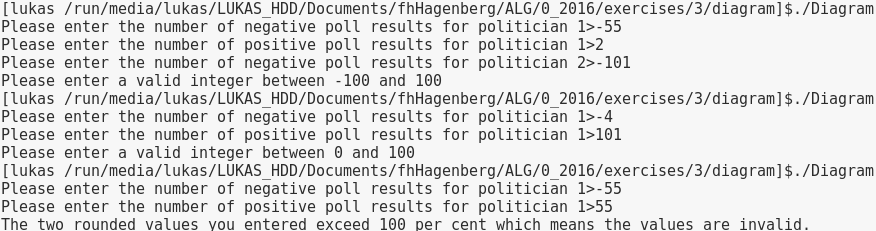
\includegraphics[scale=0.40]{diagram/tests/invalidInputs.png}
				\caption{Korrektes Verhalten bei Fehleingaben}
				\label{diagramInvalidInputs}
			\end{figure}
		\end{center}
		
		\clearpage
		Danach werden erlaubte Extremwerte (-100\% und 100\%) für beide Politiker eingegeben. Das korrekte Ergebnis ist in Abbildung \ref{diagramExtremeValues} zu sehen.
		\begin{center}
			\begin{figure}[ht!]
				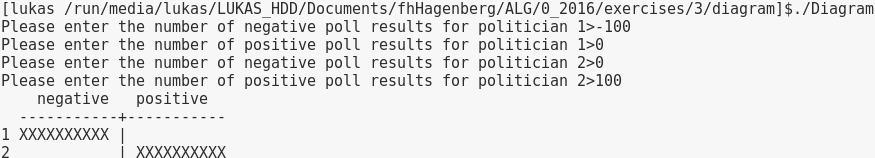
\includegraphics[scale=0.40]{diagram/tests/extremeValues.png}
				\caption{Eingabe von Extremwerten}
				\label{diagramExtremeValues}
			\end{figure}
		\end{center}
		
		Abschließend werden nicht-extreme reguläre Werte eingegeben. Wie im Screenshot \ref{diagramRegularValues} zu sehen ist, verbraucht die grafische Darstellung nun weniger Platz.
		
		\begin{center}
			\begin{figure}[ht!]
				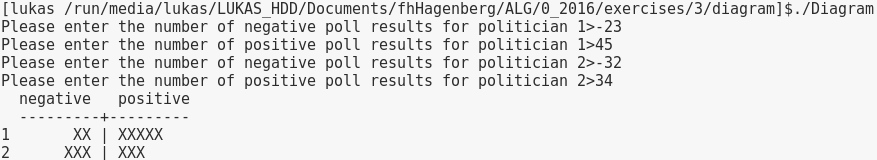
\includegraphics[scale=0.40]{diagram/tests/regularValues.png}
				\caption{Eingabe von Extremwerten}
				\label{diagramRegularValues}
			\end{figure}
		\end{center}
		
		\clearpage
		\item
		\section*{Lösungsidee}
		Zuerst wird die Gaußsche Summenformel angewandt, um mittels n die Summe, welche das Ergebnis der Reihe zu berechnen. Danach werden die Werte des Eingabefeldes durchlaufen und summiert. Das fehlende Element ist die Differenz zwischen der Gaußschen Summenformel und der Summe der Eingabewerte.
		
		\section*{Implementierung}
		\begin{lstlisting}[label=scMissingElement, resetmargins=true]
CONST MAX_ELEMENTS = 100;

TYPE IntArray = ARRAY[1..MAX_ELEMENTS] OF INTEGER;

(* Searches the missing element in a row of unsorted numbers *)
FUNCTION MissingElement(VAR a: IntArray; n: INTEGER): INTEGER;
  VAR sum: INTEGER;
    arraySum: INTEGER;
    i: SMALLINT;
BEGIN
  IF n > 0 THEN BEGIN
    (* use a sum formula for determining the sum of the row *)
    sum := ((n + 1) * (n + 2)) DIV 2;
    
    (* calculate the sum of the row excluding the missing element *)
    FOR i := 1 TO n DO BEGIN
      arraySum := arraySum + a[i];
    END;
    (* determine the missing element *)
    MissingElement := (sum - arraySum);
    END
  ELSE BEGIN
    MissingElement := (-1);
  END;
END;
		\end{lstlisting}
		
		\clearpage
		\section*{Testfälle}
		Zuerst wird überprüft, ob die Funktion den Wert (-1) für Eingaben mit weniger als einem Element zurückliefert. Dazu wird die Funktion wie unten zu sehen ist aufgerufen.
		\begin{lstlisting}
PROGRAM MissingElementTest;
VAR testElements: IntArray;

BEGIN	
  WriteLn(MissingElement(testElements, 0));
END.
		\end{lstlisting}
		Das Ergebnis ist -1, wie in Screenshot \ref{missingElementInvalidInput} ersichtlich ist.
		\begin{center}
			\begin{figure}[ht!]
				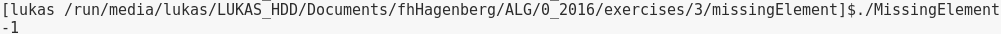
\includegraphics[scale=0.40]{missingElement/test/0input.png}
				\caption{Ergebnis bei n = 0}
				\label{missingElementInvalidInput}
			\end{figure}
		\end{center}
		
		Der Test der eigentlichen Funktion wird mit geraden und ungeraden Werten für n durchgeführt, sowie mit unterschiedlichen fehlenden Werten, welche wieder gerade und ungerade sind.
		
		\begin{lstlisting}
  testElements[1] := 3;
  testElements[2] := 2;
  testElements[3] := 4;
  testElements[4] := 5;
  WriteLn(MissingElement(testElements, 4));

  testElements[1] := 3;
  testElements[2] := 2;
  testElements[3] := 4;
  testElements[4] := 1;
  WriteLn(MissingElement(testElements, 4));

  testElements[1] := 3;
  testElements[2] := 2;
  testElements[3] := 1;
  testElements[4] := 5;
  WriteLn(MissingElement(testElements, 4));

  testElements[1] := 5;
  testElements[2] := 2;
  testElements[3] := 4;
  testElements[4] := 1;
  testElements[5] := 6;
  WriteLn(MissingElement(testElements, 5));
		\end{lstlisting}
		
		Die Ergebnisse dieser sind in Abbildung \ref{missingElements} ersichtlich.
		\begin{center}
			\begin{figure}[ht!]
				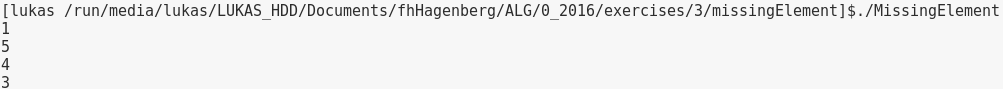
\includegraphics[scale=0.40]{missingElement/test/missingElements.png}
				\caption{Die Ausgabe der gesuchten Elemente.}
				\label{missingElements}
			\end{figure}
		\end{center}
	\end{enumerate}
\end{document}
